% {{{ Preamble ----------------------------------------------------------------
\documentclass{beamer}
\usepackage{pdfpages}

% encodings, fonts etc.
\usepackage[utf8x]{inputenc}
\usepackage[T1]{fontenc}

% math packages
\usepackage{amsmath, amssymb, amsthm}
\usepackage{mathtools}

% beamer configuration
\usetheme{Copenhagen}
%\usetheme{metropolis}
\beamertemplatenavigationsymbolsempty
%\setbeamertemplate{theorems}[numbered]
\setbeamersize{description width=2.0em}

%\usepackage{pgfpages}
%\setbeameroption{show notes}
%\setbeameroption{show notes on second screen=right}

% algorithms
\usepackage{algorithm}
\usepackage[noend]{algpseudocode}

% misc. packages
\usepackage{float}
\usepackage{varwidth}
\usepackage{listings}
\lstset{
  %breaklines=true,
  keepspaces=true,
  %frame=ltrb,
  %framesep=1pt,
  %commentstyle=\color{grey},
  basicstyle=\ttfamily\tiny,
  numbers=left,
  title=\lstname,
  columns=fullflexible,
  inputencoding=utf8,
  extendedchars=true,
}

% graphics and tikz
\usepackage{pgf}
\usepackage{tikz}
\usetikzlibrary{positioning,arrows,calc}
\tikzset{
    on grid,
    node distance=3cm,
    auto,
    block/.style = {
        draw,
        shape=rectangle,
        minimum height=3em,
        minimum width=3em,
        line width=1pt
    },
    control/.style = {
        draw,
        shape=circle,
        minimum height=7em,
        minimum width=3em,
        line width=1pt
    },
    mux/.style = {
        draw,
        shape=rectangle,
        minimum height=1.5em,
        minimum width=1em,
        line width=1pt
    },
    empty/.style = {
        shape=rectangle,
        minimum height=3em,
        minimum width=3em
    },
    >=latex',
}


% mathematics
\newtheorem{proposition}{Proposition}

\renewcommand{\tt}{\texttt}

% title page
\title{Implementing a MIPS processor using SME}
\author[Carl-Johannes Johnsen]{
  \mbox{Carl-Johannes Johnsen}}
\institute{Department of Computer Science\\
           University of Copenhagen}
%\date{December 22, 2016}
% }}} -------------------------------------------------------------------------

\begin{document}

% {{{ Title page --------------------------------------------------------------
\frame{\titlepage}
% }}} -------------------------------------------------------------------------

% {{{ Table of contents -------------------------------------------------------
%\begin{frame}
%  \frametitle{Outline}
%  \tableofcontents
%\end{frame}
% }}} -------------------------------------------------------------------------


\begin{frame}{Background}
  The Machine Architecture class at DIKU taught the theory of computer organization and design. However, it did not teach how to construct specialized hardware, as one might implement on an FPGA.

  \vspace{\baselineskip}
  FPGAs are more attractive than general purpose CPUs in some applications, as they do not necessarily have the same overhead in both performance and power usage, as they are not as complex.

  \vspace{\baselineskip}
  However, FPGAs are programmed using Hardware Description Languages, which are very tedious to program. This has changed with SME.
\end{frame}

\begin{frame}{Introduction}
  The SME programming model is similar to the CSP model, except it is globally synchronous, has broadcasting channels and a hidden clock. This makes it more suitable for generating hardware models than CSP. Additionally, SME can be transpiled into VHDL, which can be written onto an FPGA.

  \vspace{\baselineskip}
  I am implementing a MIPS processor as taught in Machine Architecture by using SME, and documenting the process, so it could be used as teaching material for a course on hardware development.
\end{frame}

\begin{frame}{Basic combinatorial}
  I started by implementing some basic combinatorial circuits, as this was an simple approach to SME. The first one I made consisted of four processes, which simulate four basic gates: AND, NOT, OR and XOR.

  \vspace{\baselineskip}
  Then I connected these into networks: an decoder, a half adder and a full adder.
\end{frame}

\begin{frame}[fragile]{Basic combinatorial - Full adder example}
  \begin{columns}
    \begin{column}{.48\textwidth}
      \begin{lstlisting}
public interface InputA : IBus {
    bool bit { get; set; }
}
...
public class AndGate : SimpleProcess {
  [InputBus] InputB input1;
  [InputBus] InputC input2;
  [OutputBus] Internal3 output;

  protected override void OnTick() {
    output.bit = input1.bit && input2.bit;
  }
}

public class OrGate : SimpleProcess {
  ...
  protected override void OnTick() {
    output.bit = input1.bit || input2.bit;
  }
}

public class XorGate : SimpleProcess {
  ...
  protected override void OnTick() {
    output.bit = input1.bit ^ input2.bit;
  }
}
\end{lstlisting}
    \end{column}
    \begin{column}{.48\textwidth}
      \begin{figure}
          \centering
          \scalebox{0.5}{
            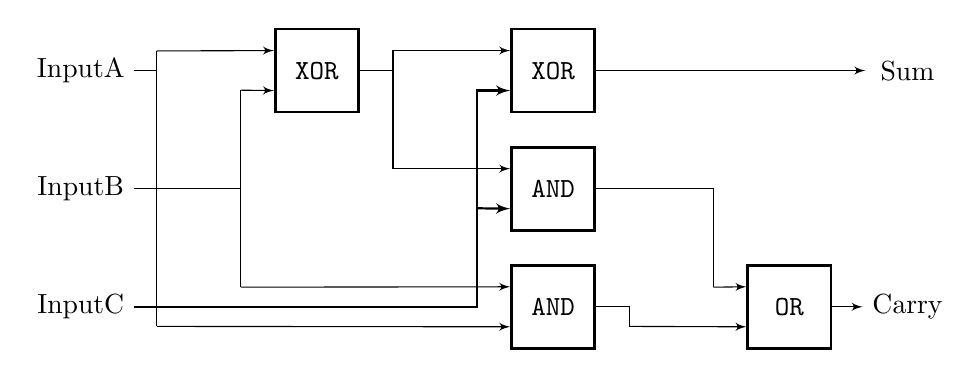
\begin{tikzpicture}[node distance=1.5cm]
                \node[block] (or) {\texttt{OR}};
                \node[empty, left of=or] (orin) {};
                \node[block, left of=orin] (and1) {\texttt{AND}};
                \node[block, above of=and1] (and0) {\texttt{AND}};
                \node[empty, left of=and0] (and0in) {};
                \node[block, above of=and0] (xor1) {\texttt{XOR}};
                \node[empty, left of=xor1] (xor1in) {};
                \node[block, left of=xor1in] (xor0) {\texttt{XOR}};
                \node[empty, left of=xor0] (xor0in) {};
                \node[empty, left of=xor0in] (inputa) {InputA};
                \node[empty, below of=inputa] (inputb) {InputB};
                \node[empty, below of=inputb] (inputc) {InputC};
                \node[empty, right of=inputc] (inputcout) {};
                \node[empty, right of=xor1] (sum) {};
                \node[empty, right of=sum] (summ) {};
                \node[empty, right of=summ] (summm) {Sum};
                \node[empty, right of=or] (carry) {Carry};

                \path[draw, -] (inputa.east) -| (xor0in.155);
                \path[draw, ->] (xor0in.155) -- (xor0.155);
                \path[draw, -] (inputb.east) -| (xor0in.335);
                \path[draw, ->] (xor0in.335) -- (xor0.205);

                \path[draw, -] (inputa.east) -| (inputcout.205);
                \path[draw, ->] (inputcout.205) -- (and1.205);
                \path[draw, -] (inputb.east) -| (inputcout.25);
                \path[draw, ->] (inputcout.25) -- (and1.155);

                \path[draw, thick, -] (inputc.east) -| (and0in.335);
                \path[draw, thick, ->] (and0in.335) -- (and0.205);
                \path[draw, thick, ->] (and0in.335) |- (xor1.205);

                \path[draw, -] (xor0.east) -- (xor1in.west);
                \path[draw, ->] (xor1in.west) |- (xor1.155);
                \path[draw, ->] (xor1in.west) |- (and0.155);

                \path[draw, -] (and1.east) -| (orin.205);
                \path[draw, ->] (orin.205) -- (or.205);
                \path[draw, ->] (xor1) -- (summm);
                \path[draw, -] (and0.east) -| (orin.25);
                \path[draw, ->] (orin.25) -- (or.155);
                \path[draw, ->] (or) -- (carry);
            \end{tikzpicture}
          }
          \label{fig:full-adder}
      \end{figure}
    \end{column}
  \end{columns}
\end{frame}

\begin{frame}[fragile]{Components}
  After getting some experience with SME, i started working on the MIPS processor. I started by implementing each of the components as SME processes, as I can then verify them individually.

  \vspace{\baselineskip}
  \begin{lstlisting}
public class Register : SimpleProcess {
  ...
  uint[] data = new uint[32];

  protected override void OnTick() {
    if (write.enabled && write.addr > 0)
      data[write.addr] = write.data;
    outputA.data = data[readA.addr];
    outputB.data = data[readB.addr];
  }
}
\end{lstlisting}
\end{frame}

\begin{frame}{Single Cycle}
  With all of the components implemented and verified, 'wiring' up the processes is straightforward, as the busses should just be named accordingly.

  \begin{figure}
        \centering
        \scalebox{0.5}{
            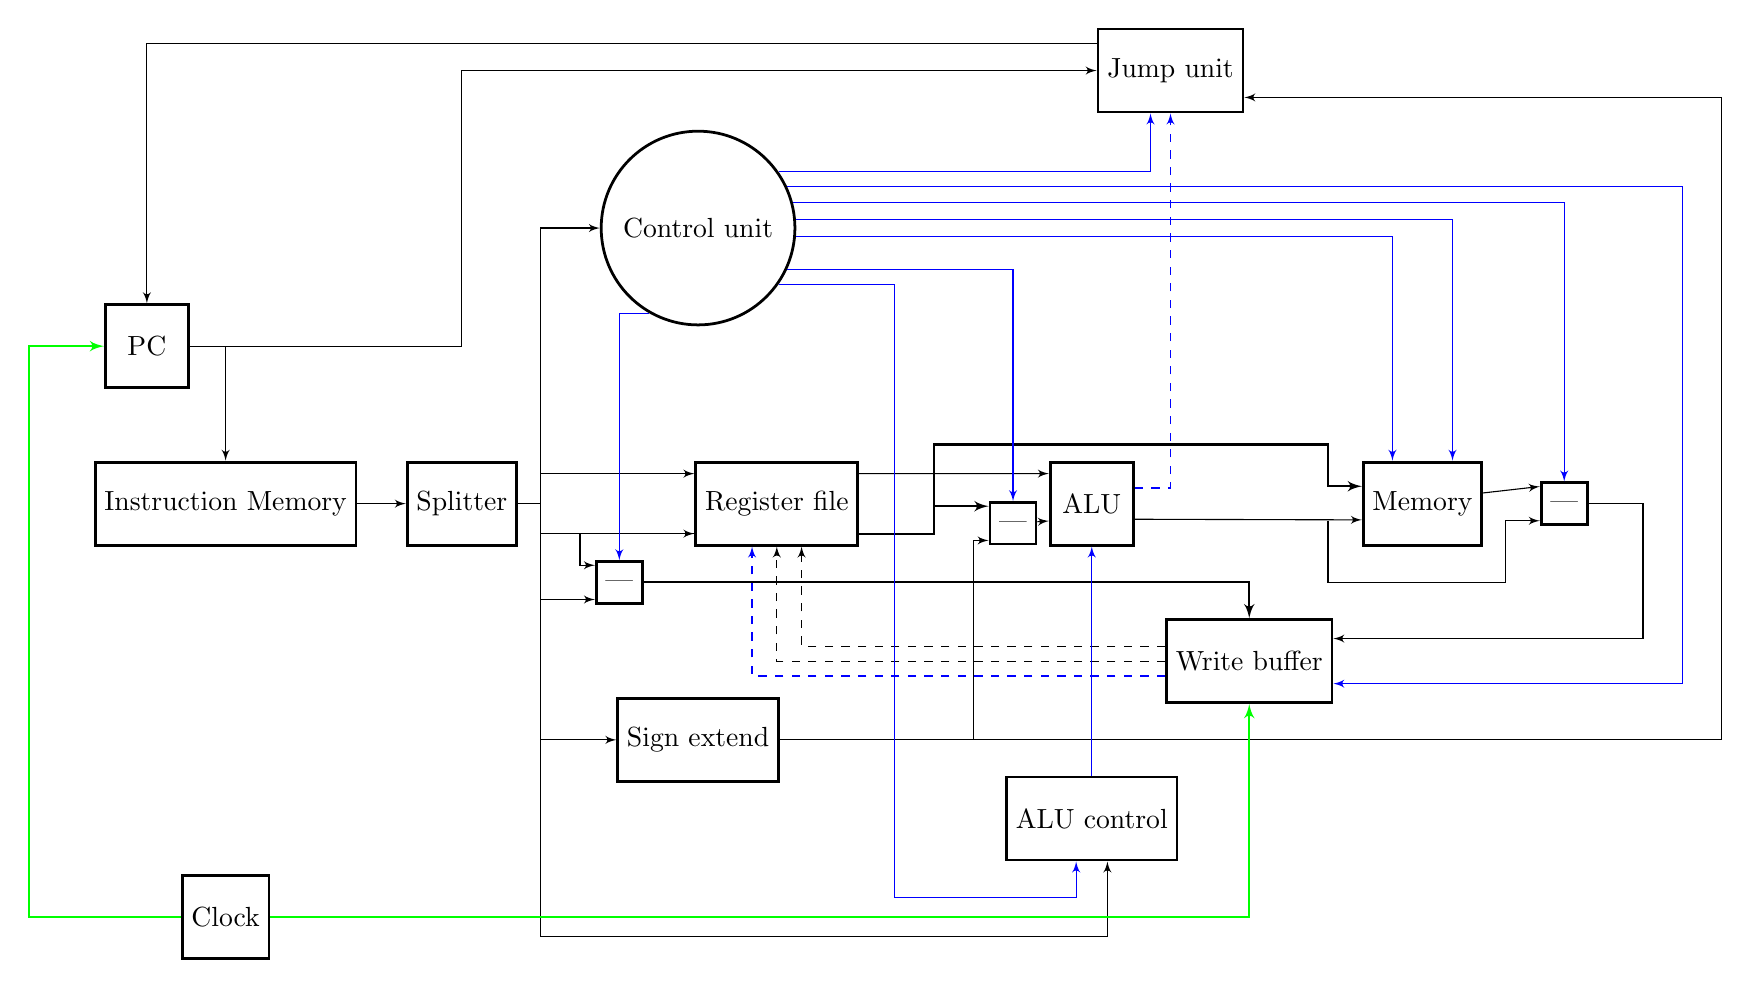
\begin{tikzpicture}
                \node[block] (reg) at (0,0) {Register file};
                \node[control] (cont) at (-1,3.5) {Control unit};
                \node[block] (jump) at (5,5.5) {Jump unit};
                \node[empty] (splitspace) at (-3,0) {};
                \node[block] (split) at (-4,0) {Splitter};
                \node[block] (if) at (-7,0) {Instruction Memory};
                \node[block] (sign) at (-1,-3) {Sign extend};
                \node[block] (alu) at (4,0) {ALU};
                \node[block] (alucont) at (4,-4) {ALU control};
                \node[block] (mem) at (8.2,0) {Memory};
                \node[mux] (memread) at (10,0) {|};
                \node[mux] (imm) at (3, -0.25) {|};
                \node[mux] (regdst) at (-2,-1) {|};
                \node[block] (pc) at (-8, 2) {PC};
                \node[block] (writebuf) at (6, -2) {Write buffer};

                \path[draw, ->] (if) -- (split);
                \path[draw, -] (split) -- (splitspace.center);
                \path[draw, ->] (splitspace.center) |- (sign);
                \path[draw, ->] (splitspace.center) |- (cont);
                \path[draw, ->] (splitspace.center) |- (reg.160);
                \path[draw, ->] (splitspace.center) |- (reg.200);
                %\path[draw, ->] (splitspace.center) |- (alucont.200);
                \path[draw, ->] (splitspace.center) |- (2,-5.5) -| (alucont.290);
                \path[draw, ->] (splitspace.center) |- (regdst.215);
                \path[draw, ->] (reg.200) -| (-2.5, -0.5) |- (regdst.145);
                %\path[draw, ->] (alucont) -| (12.5, 0) |- (jump);
                \path[draw, thick, ->] (reg.340) -| (2,-0.25) |- (imm.145);
                \path[draw, thick, ->] (2,-0.25) |- (3,0.75) -- (7,0.75) |-
                (mem.164);
                \path[draw, ->] (reg.20) -- (alu.145);
                \path[draw, ->, dashed, color=blue] (alu.20) -| (jump);
                %\path[draw, ->] (alu.340) -- (jal);
                %\path[draw, ->] (jal) -- (mem.196);
                %\path[draw, ->] (jal) -- (writebuf);
                \path[draw, ->] (alu.340) -- (mem.195);
                \path[draw, ->] (imm) -- (alu.202);
                \path[draw, ->] (7, -0.22) |- (8, -1) -| (9.25,-0.5) |-
                (memread.215);
                \path[draw, ->] (mem.10) -- (memread.145);
                \path[draw, ->] (sign) -| (2.5, -1) |- (imm.215);
                \path[draw, ->] (2.5,-3) -| (12, 0) |- (jump.340);
                %\path[draw, thick, ->] (regdst) -| (5, -0.6) |- (jal.210);
                \path[draw, thick, ->] (regdst) -| (writebuf);
                \path[draw, ->] (pc) -| (if);
                \path[draw, ->] (pc) -| (-4, 4) |- (jump);
                \path[draw, ->] (jump.160) -| (pc);
                \path[draw, ->] (memread) -| (11, -1) |- (writebuf.15);
                \path[draw, dashed, ->] (writebuf.170) -| (reg.300);
                \path[draw, dashed, ->] (writebuf) -| (reg);
                \path[draw, dashed, ->, color=blue] (writebuf.190) -| (reg.240);

                \path[draw, ->, color=blue] (alucont) -- (alu);
                \path[draw, ->, color=blue] (cont.35) -| (jump.245);
                \path[draw, ->, color=blue] (cont.25) -| (11.5,0) |-
                (writebuf.345);
                \path[draw, ->, color=blue] (cont.15) -| (memread);
                \path[draw, ->, color=blue] (cont.5) -| (mem.55);
                \path[draw, ->, color=blue] (cont.355) -| (mem.125);
                \path[draw, ->, color=blue] (cont.335) -| (imm);
                \path[draw, ->, color=blue] (cont.325) -| (1.5, -4) |-
                (2, -5) -| (alucont.250);
                \path[draw, ->, color=blue] (cont.240) -| (regdst);

                \node[block] (clock) at (-7, -5.25) {Clock};
                \path[draw, ->, thick, color=green] (clock) -| (-9.5,0) |- (pc);
                \path[draw, ->, thick, color=green] (clock) -| (writebuf);
            \end{tikzpicture}
        }
  \end{figure}
\end{frame}

\begin{frame}{Pipelining}
  Following the procedure from the Machine Architecture class, I have pipelined the processor, and handled the hazards introduced by pipelining with an hazard detection unit, and a forwarding unit.

  \begin{figure}
        \centering
        \scalebox{0.5}{
            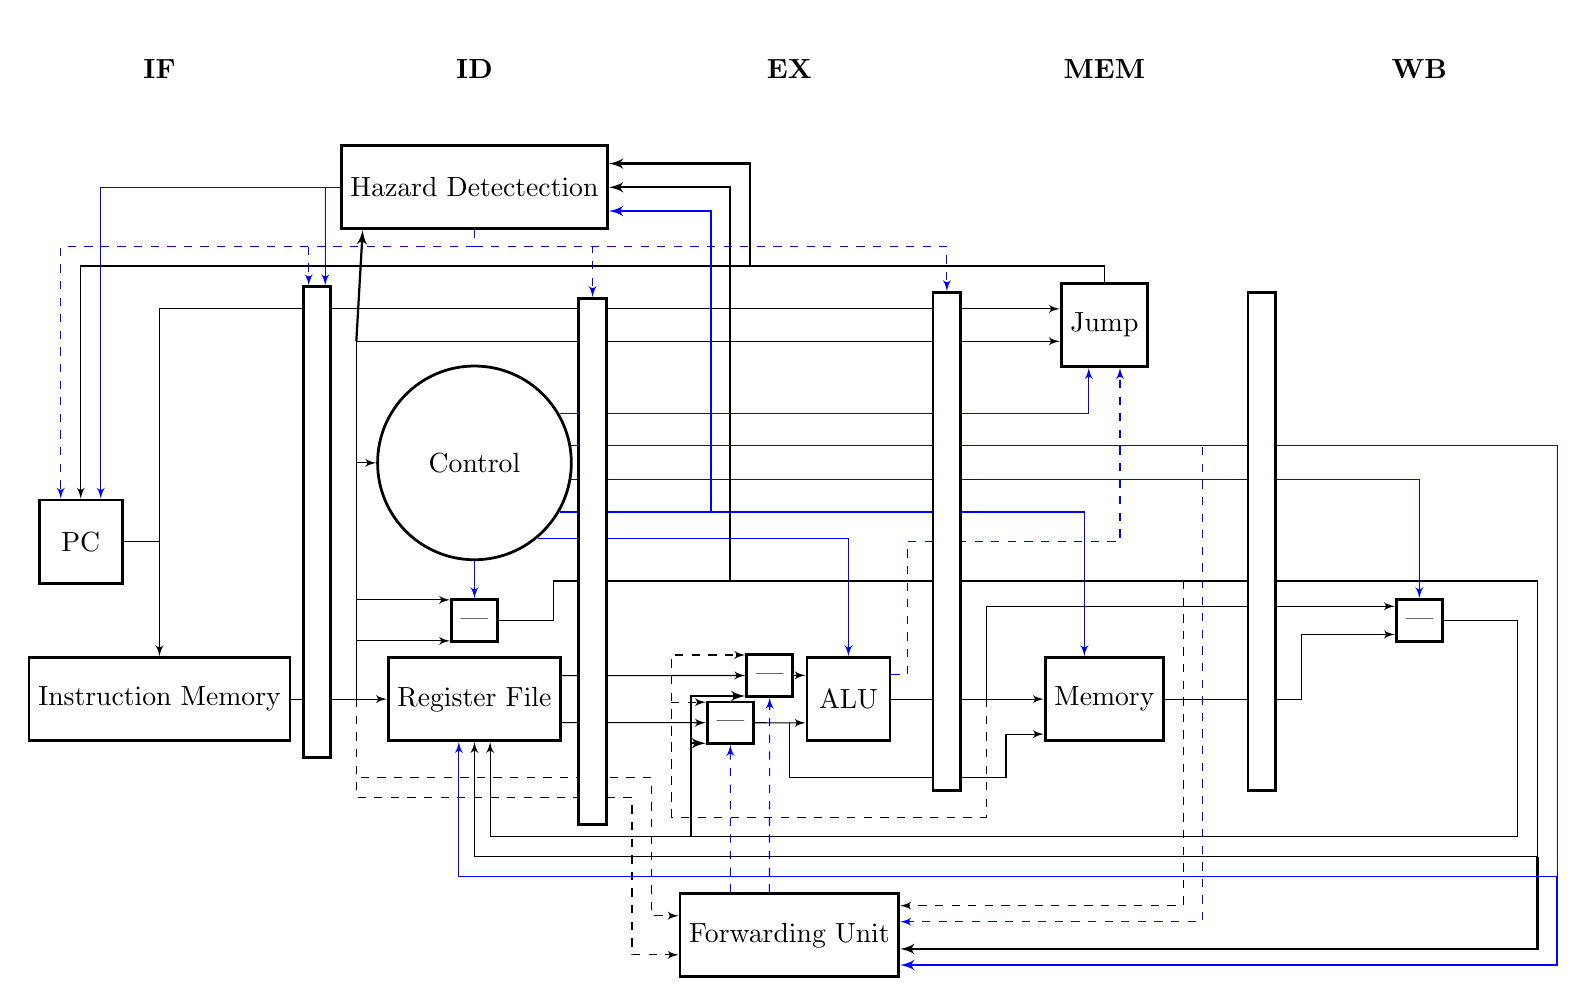
\begin{tikzpicture}
                \node[block] (alu) at (0.75,0) {ALU};
                \node[block] (reg) at (-4,0) {Register File};
                \node[block] (memo) at (4,0) {Memory};
                \node[block] (jump) at (4,4.75) {Jump};
                \node[block] (imem) at (-8,0) {Instruction Memory};
                \node[block] (pc) at (-9, 2) {PC};
                \node[control] (cont) at (-4, 3) {Control};
                \node[mux] (wbm) at (8,1) {|};
                \node[block] (forw) at (0, -3) {Forwarding Unit};
                \node[mux] (forwa) at (-0.25, 0.3) {|};
                \node[mux] (forwb) at (-0.75, -0.3) {|};
                \node[mux] (addr) at (-4, 1) {|};
                \node[block] (haz) at (-4,6.5) {Hazard Detectection};

                \node[empty] (if) at (-8, 8) {\textbf{IF}};
                \node[empty] (id) at (-4, 8) {\textbf{ID}};
                \node[empty] (ex) at (0, 8) {\textbf{EX}};
                \node[empty] (mem) at (4, 8) {\textbf{MEM}};
                \node[empty] (wb) at (8, 8) {\textbf{WB}};

                \path[draw, ->] (pc) -| (imem);
                \path[draw, ->] (imem) -- (reg);
                \path[draw, ->] (-5.5,0) |- (cont);
                \path[draw, ->] (-5.5,0) |- (addr.220);
                \path[draw, ->] (-5.5,0) |- (addr.140);
                %\path[draw, ->] (reg.15) -- (alu.151);
                \path[draw, ->] (reg.15) -- (forwa);
                \path[draw, ->] (forwa) --  (alu.151);
                \path[draw, ->] (reg.345) -- (forwb);
                \path[draw, ->] (forwb) -- (alu.209);
                \path[draw, ->] (alu) -- (memo);
                \path[draw, ->] (0,-0.3) |- (0,-1) -- (2.75,-1) |- (memo.210);
                \path[draw, ->] (2.5, 0) |- (wbm.150);
                \path[draw, ->] (memo) -- (6.5, 0) |- (wbm.210);
                \path[draw, ->] (wbm) -| (9.25, -1.75) -| (reg.290);
                \path[draw, color=blue, dashed, ->] (alu.30) -| (1.5,1) |- (4,2) -| (jump.290);
                \path[draw, ->] (jump) |- (0,5.5) -| (pc);
                \path[draw, ->] (-8,2) |- (jump.160);
                \path[draw, ->] (-5.5,3) |- (jump.200);
                \path[draw, thick, ->] (-1.25,-1.75) |- (forwb.220);
                \path[draw, thick, ->] (-1.25,-1.75) |- (forwa.220);
                \path[draw, dashed, ->] (2.5, 0) |- (-1.5, -1.5) |- (forwb.140);
                \path[draw, dashed, ->] (-1.5, -1.5) |- (forwa.140);
                \path[draw, ->] (addr) -| (-3, 1.5) -| (9.5,-2) -|
                (reg.270);
                \path[draw, thick, ->] (9.5, -2) |- (forw.353);
                \path[draw, dashed, ->] (5,1.5) |- (forw.15);
                \path[draw, dashed, ->] (-5.5,0) |- (-1.75,-1) |- (forw.170);
                \path[draw, dashed, ->] (-5.5,0) |- (-2,-1.25) |- (forw.190);

                \path[draw, color=blue, ->] (cont.310) -| (alu);
                \path[draw, color=blue, ->] (cont.330) -| (memo.115);
                \path[draw, color=blue, ->] (cont.350) -| (wbm);
                \path[draw, color=blue, ->] (cont.10) -| (9.75,-2.25) -| (reg.250);
                \path[draw, color=blue, ->] (cont.30) -| (jump.250);
                \path[draw, color=blue, ->] (cont) -- (addr);
                \path[draw, color=blue, thick, ->] (9.75,-2.25) |- (forw.345);
                \path[draw, color=blue, dashed, ->] (5.25, 3.2) |- (forw.7);

                \path[draw, color=blue, dashed, ->] (forw.115) -- (forwa);
                \path[draw, color=blue, dashed, ->] (forw.144) -- (forwb);

                % Hazard
                \path[draw, thick, ->] (-0.75, 1.5) |- (haz); % addr
                \path[draw, thick, color=blue, ->] (-1, 2.37) |- (haz.350); % mem
                \path[draw, thick, ->] (-0.5, 5.5) |- (haz.10); % pcsrc
                \path[draw, thick, ->] (-5.5, 4.55) -- (haz.201);% reada readb
                \path[draw, dashed, color=blue, -] (haz) -- (-4, 5.75);

                \node[block, minimum height=170, minimum width=10, fill=white] (ifid) at
                (-6,2.25) {};
                \node[block, minimum height=190, minimum width=10, fill=white] (idex) at
                (-2.5,1.75) {};
                \node[block, minimum height=180, minimum width=10, fill=white]
                (exmem) at (2,2) {};
                \node[block, minimum height=180, minimum width=10, fill=white]
                (memwb) at (6,2) {};

                \path[draw, dashed, color=blue, ->] (-4, 5.75) -| (exmem);
                \path[draw, dashed, color=blue, ->] (-4, 5.75) -| (idex);
                \path[draw, dashed, color=blue, ->] (-4, 5.75) -| (ifid.92);
                \path[draw, dashed, color=blue, ->] (-4, 5.75) -| (pc.115);
                \path[draw, color=blue, ->] (haz) -| (ifid.88);
                \path[draw, color=blue, ->] (haz) -| (pc.65);
            \end{tikzpicture}
        }
        \label{fig:hazard}
    \end{figure}
\end{frame}

\begin{frame}{Performance}
  To test both the single cycle processor and the pipelined processor, I have made some programs in MIPS assembler. To verify both the number of executed clock ticks and the results of the program, I have run them in the MIPS simulation program MARS.
  \begin{table}
    \centering
    \scalebox{0.75}{
      \begin{tabular}{rlllllllllll}
          \hline
          & & \# CT \texttt{MARS} & \# CT & time (ms) & clockrate (hz) \\
          \hline
          Towers of Hanoi & $n=5$ &
              719 & 720 - 1058 & 516 - 1190 & $\sim$1395 - $\sim$889 \\

          Quicksort & $n=8$ &
              483 & 484 - 763 & 375 - 895 & $\sim$1290 - $\sim$852 \\

          Fibonacci & $n=10$ &
              85 & 86 - 126 & 113 - 212 & $\sim$761 - $\sim$594 \\
          \hline
      \end{tabular}
    }
    \label{tab:perf-pipe}
  \end{table}
\end{frame}

\begin{frame}{Synthesizing}
  As mentioned SME can be transpiled into VHDL. Once the VHDL has been transpiled, it can be simulated by \texttt{ghdl}, in order to get a quick pointer on the correctness of the transpiled code. Once the code has passed simulation, it can be synthesized and implemented on a FPGA with the use of FPGA tools.

  \vspace{\baselineskip}
  This is as far as I am with the project. So far, I have succesfully generated VHDL for all of the basic combinatorial networks, individual components and the single cycle processor. However, the processor fails synthesization.
\end{frame}

\begin{frame}{Synthesizing - Single cycle processor RTL}
  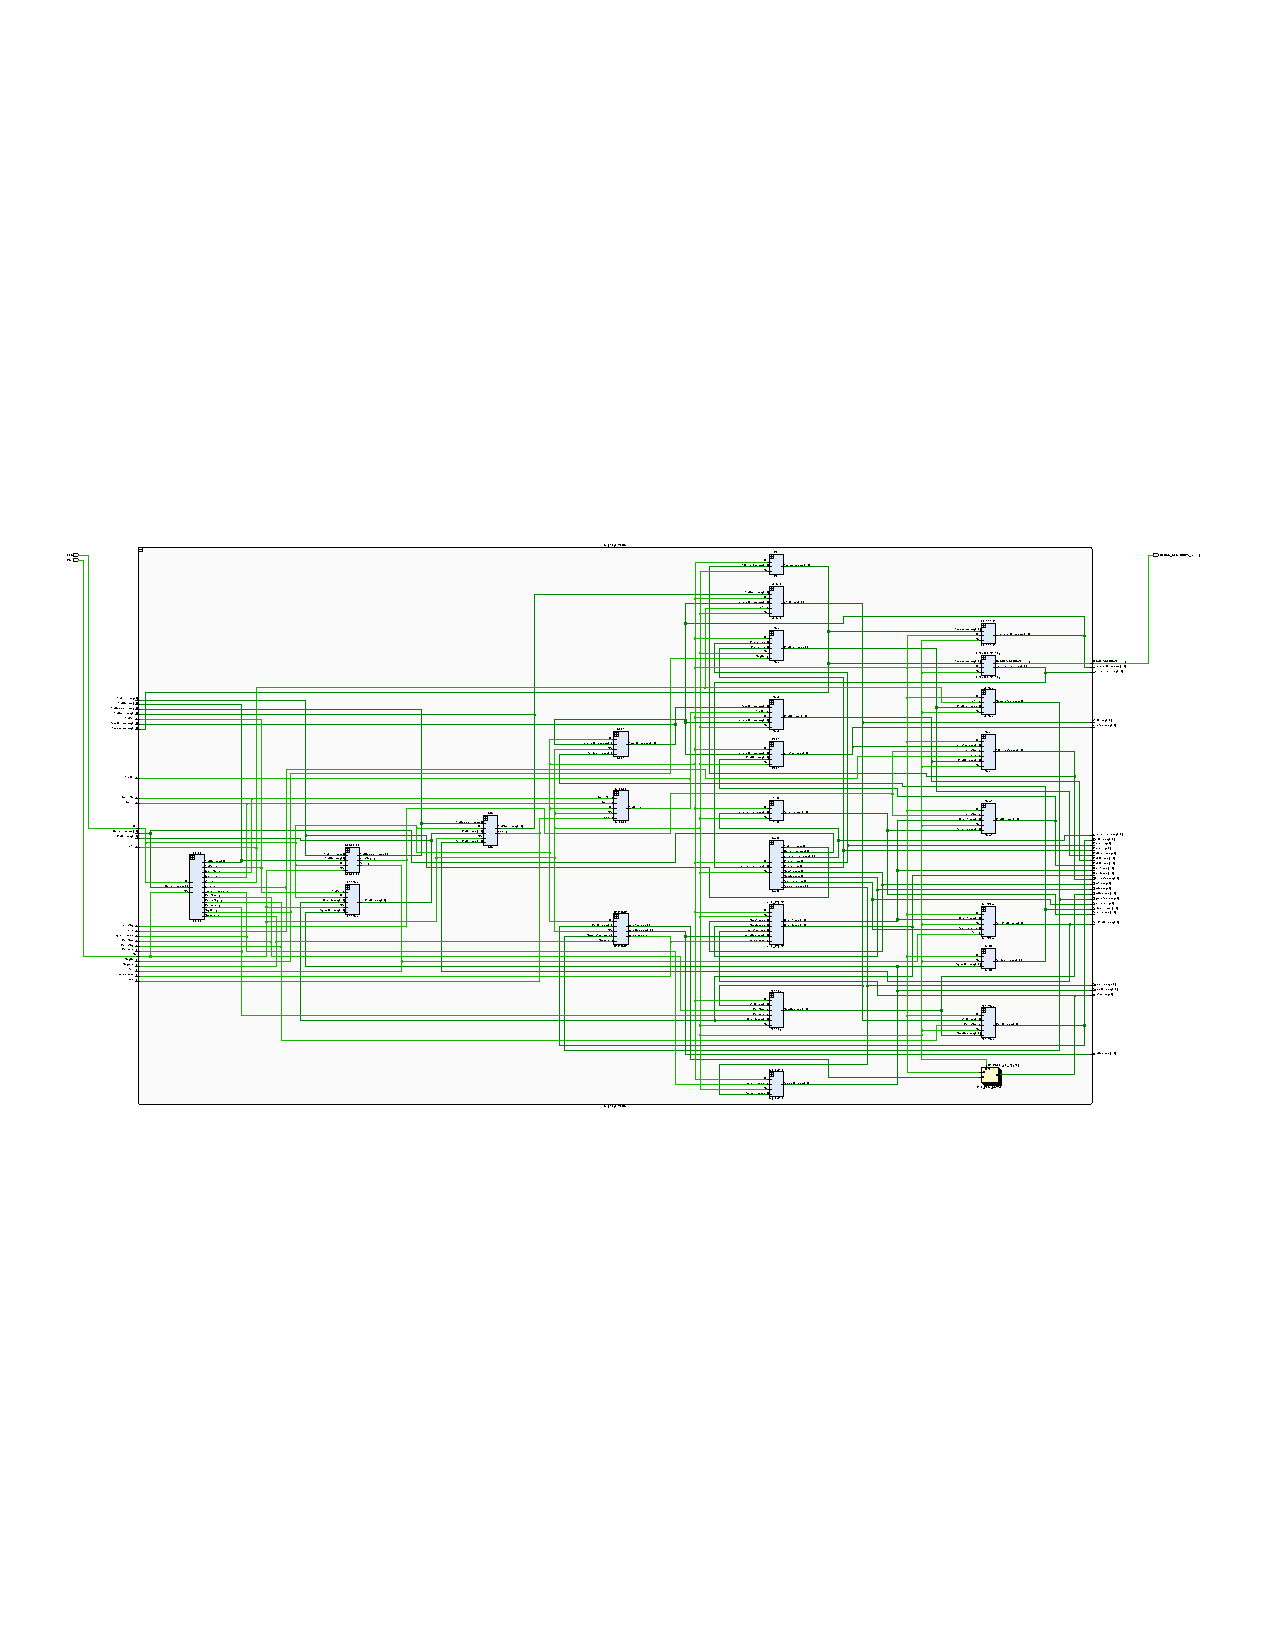
\includegraphics[width=\textwidth,height=\textheight]{SingleCycleRTL.pdf}
\end{frame}

\begin{frame}{Synthesizing - Logic gates}
  I have only managed to fully implement the first SME network, which consisted of the four basic gates.
  \includegraphics[width=.24\textwidth]{FF2}
  \includegraphics[width=.24\textwidth]{FT2}
  \includegraphics[width=.24\textwidth]{TF2}
  \includegraphics[width=.24\textwidth]{TT2}
\end{frame}

\begin{frame}{Future Work}
  \begin{itemize}
    \item Synthesize and write single cycle processor to FPGA
    \item Synthesize and write the pipelined processor to FPGA
    \item Fit more cores onto a single FPGA
    \item Introduce multiple execution paths
  \end{itemize}
\end{frame}

% exit section
\AtBeginSection{}
\section*{}

% {{{ Bibliography ------------------------------------------------------------
%\begin{frame}{Bibliography}
%  \tiny
%  \bibliographystyle{plain}
%  \bibliography{pl}
%\end{frame}
% }}} -------------------------------------------------------------------------

\end{document}
